\documentclass[a4paper,12pt]{article} 

%%% Работа с русским языком
\usepackage{cmap}					% поиск в PDF
\usepackage{mathtext} 				% русские буквы в фомулах
\usepackage[T2A]{fontenc}			% кодировка
\usepackage[utf8]{inputenc}			% кодировка исходного текста
\usepackage[english,russian]{babel}	% локализация и переносы

%%% Дополнительная работа с математикой
\usepackage{amsmath,amsfonts,amssymb,amsthm,mathtools, gensymb} % AMS
\usepackage{icomma} % "Умная" запятая: $0,2$    ф--- число, $0, 2$ --- перечисление

%%Таблица
\usepackage[table,xcdraw]{xcolor}
\usepackage{caption}
\usepackage{floatrow}
\floatsetup[table]{capposition=top}
\floatsetup[wrapfigure]{capposition=bottom}
\usepackage{multirow}

%Отступы и поля 
\textwidth=18cm
\oddsidemargin=-1cm
\topmargin=-2cm
\textheight=25cm


%% Номера формул
\mathtoolsset{showonlyrefs=true} % Показывать номера только у тех формул, на которые есть \eqref{} в тексте.

%% Шрифты
\usepackage{euscript}	 % Шрифт Евклид
\usepackage{mathrsfs} % Красивый матшрифт

%% Свои команды
\DeclareMathOperator{\sgn}{\mathop{sgn}}

%% Перенос знаков в формулах (по Львовскому)
\newcommand*{\hm}[1]{#1\nobreak\discretionary{}
{\hbox{$\mathsurround=0pt #1$}}{}}

%% Стиль страницы
\usepackage{fancyhdr}

%% Для рисунков
\usepackage{graphicx}
\usepackage[export]{adjustbox}
\usepackage{float}
\usepackage{ragged2e}
\usepackage{wrapfig}

\pagestyle{fancy}
\begin{document}
\begin{titlepage}
\begin{center}
%\vspace*{1cm}
\large{\small ФЕДЕРАЛЬНОЕ ГОСУДАРСТВЕННОЕ АВТОНОМНОЕ ОБРАЗОВАТЕЛЬНОЕ\\ УЧРЕЖДЕНИЕ ВЫСШЕГО ОБРАЗОВАНИЯ \\ МОСКОВСКИЙ ФИЗИКО-ТЕХНИЧЕСКИЙ ИНСТИТУТ\\ (НАЦИОНАЛЬНЫЙ ИССЛЕДОВАТЕЛЬСКИЙ УНИВЕРСИТЕТ)\\ ФАКУЛЬТЕТ АЭРОКОСМИЧЕСКИХ ТЕХНОЛОГИЙ}
\vfill
\line(1,0){490}\\[1mm]
\huge{Лабораторная работа 4.3.3}\\
\huge\textbf{Исследование разрешающей способности микроскопа методом Аббе}\\
\line(1,0){490}\\[1mm]
\vfill
\begin{flushright}
\normalsize{Рогозин Владимир}\\
\normalsize{\textbf{Группа Б03-106}}\\
\end{flushright}
\end{center}
\end{titlepage}
\fancyhead[L] {Работа 4.3.3}

\textbf{Цель работы}:
изучение дифракционного предела разрешения объектива микроскопа методом Аббе.


\textbf{Оборудование}:
лазер; кассета с набором сеток разного
периода; линзы; щель с микрометрическим винтом; оптический стол
c набором рейтеров и крепёжных винтов; экран; линейка.


\section{Теоретические сведения}
Всякая оптическая система, предназначенная для получения изображений, имеет конечный предел разрешения. Принципиальной причиной, ограничивающей предел разрешения, является дифракция световых волн: ограничение пучка лучей краями линз и диафрагм, составляющих оптическую систему, приводит к нарушению \textit{стигматичности} изображения -- каждая точка предмета отображается не в одну точку, а в дифракционное пятно.Дифракционные пятна от близких точек предмета могут перекрываться друг другом, в результате чего точки становятся неразличимыми.

\textit{Разрешающей способностью оптического прибора} называют минимальное расстояние $l_{min}$ между двумя точками в пространстве предметов, изображения которых разрешаются по критерию Релея.
\begin{figure}[H]\label{fig: Microscope scheme}
    \centering
    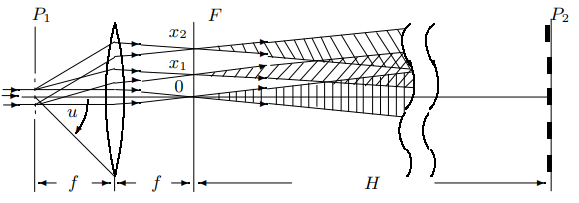
\includegraphics[width = 0.9\textwidth]{Microscope scheme.png}
    \caption{Образование изображения в объективе микроскопа}
\end{figure}

Схема образования изображения в объективе микроскопа представлена на рис. 1. Для простоты рассмотрим случай, когда предметом является периодическая структура (дифракционная решетка), освещаемая параллельным пучком лучей. При наблюдении в микроскоп предмет располагается вблизи переднего фокуса объектива.

Аббе предложил свой подход к оценке разрешающей способности: прохождение лучей от предмета к изображению разбивается на два этапа. Сначала рассматривается картина, возникающая в задней фокальной плоскости $F$ объектива (рис. 1). Эта картина называется \textit{первичным изображением} или \textit{фурье-образом} предмета. Затем первичное изображение рассматривается как источник волн, создающих изображение предмета в плоскости $P_2$ сопряженной плоскости предмета, т. е. \textit{вторичное изображение}. Такой подход основан на принципе \textit{Гюйгенса-Френеля}, согласно которому любой участок волнового фронта можно рассматривать как вторичный источник излучения.

Первичное изображение, наблюдаемое в задней фокальной плоскости объектива, представляет собой картину дифракции Фраунгофера на объекте (в нашем случае -- на дифракционной решетке). Смещение $x_m$ точки наблюдения от оптической оси связано с углом наклона $\varphi_m$ параллельного пучка лучей перед линзой соотношением (при малых $\varphi$):
$x_m \approx f \varphi_m$.   
\begin{figure}[H]\label{fig: Fraunhofer diffraction intensity}
    \centering
    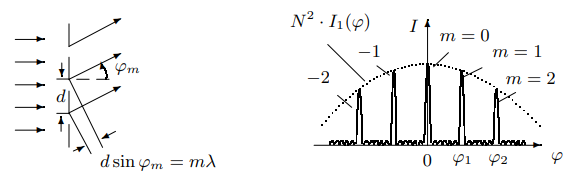
\includegraphics[width = 0.9\textwidth]{Fraunhofer diffraction intensity.png}
    \caption{Спектр амплитудной решетки. $I_1(\varphi)$ -- распределение интенсивности при дифракции света на одиночной щели, $N$ -- число щелей решетки}
\end{figure}

При дифракции Фраунгофера на одномерной решетке периода $d$ направления $\varphi_m$ 
 максимальной интенсивности (главные максимумы) определяются условием:
\begin{equation}\label{eq: max condition Fraunhofer diffraction}
     d\sin\varphi_m = m\lambda,
\end{equation}
где $\lambda$ -- длина световой волны. Главные максимумы различных порядков $m$ имеют неодинаковые интенсивности. Таким образом, первичное изображение представляет собой набор ярких точек, расположенных цепочкой на равных расстояниях друг от друга. Излучение этих когерентных точечных источников создаст в плоскости $P_2$ систему интерференционных полос, синтезирующих изображение предмет в (решётки) в этой плоскости.

При таком рассмотрении дифракционные искажения, обусловленные конечным диаметром линзы, связаны с тем, что часть первичного изображения закрывается. Через микроскоп про ходят только те пучки, для которых выполняется условие
\begin{equation}\label{eq: microscope aperture}
     \varphi_m < u,
\end{equation}
где $u$ -- \textit{апертурный угол} (рис. 1). Эти пучки лучей собираются в задней фокальной плоскости линзы, так что за ней возникают расходящиеся пучки лучей с центрами в плоскости $F$. В плоскости $P_2$ эти пучки интерферируют и воспроизводят увеличенное изображение решетки.

Для получения правильного изображения надо, чтобы через объектив микроскопа проходили дифракционные пучки разных направлений. Если апертурный угол $u$ меньше $\varphi_1$, то в плоскости $P_2$ не возникает периодического изображения. Соотношение
\begin{equation}\label{eq: Fraunhofer diffraction grid period condition}
    \sin u \geq \lambda / d
\end{equation}
можно рассматривать как условие разрешения решетки с периодом $d$. Отсюда можно найти минимальное разрешаемое объективом расстояние
\begin{equation}\label{eq: min resolving distance}
    d \geq \frac{\lambda}{\sin u} \approx \frac{\lambda}{(D / 2f)}.
\end{equation}

В данной работе применяется двумерная решетка -- сетка. Ее можно рассматривать как две скрещенные (перпендикулярные друг к другу) решетки. Узкий пучок монохроматического света, пройдя через решетку с вертикальными штрихами, дает совокупность максимумов, расположенных вдоль горизонтальной линии. Световой пучок, соответствующий каждому максимуму, проходя через вторую решетку, распадается на новую совокупность световых пучков, дающих максимумы вдоль вертикальной линии. Главные максимумы возникают тогда, когда одновременно выполняются условия:
\begin{equation}
    d\sin\varphi_x = m_x \lambda, \quad d\sin\varphi_y = m_y \lambda,
\end{equation}
где $m_x$ и $m_y$ -- целые числа, характеризующие порядки дифракционных максимумов, $\varphi_x$ и $\varphi_y$ -- направления на главные дифракционные максимумы в горизонтальной и вертикальной плоскостях соответственно. 

\begin{wrapfigure}[15]{r}{0.4\textwidth}\label{fig: Fraunhofer diffraction intensity 2D}
    \begin{center}
    \vspace{-20pt}
         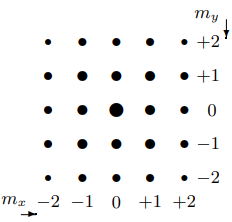
\includegraphics[width = 0.75\textwidth]{Fraunhofer diffraction intensity 2D.png}
    \end{center}
    \caption{Дифракция Фраунгофера на сетке. Максимумы изображены кружками, размеры которых характеризуют интенсивности}
\end{wrapfigure}
Максимумы, удовлетворяющие условию $\varphi_x, \varphi_y < u$, создают в задней
фокальной плоскости $F$ объектива картину дифракции Фраунгофера (рис. 3) -- первичное изображение.

Если теперь поместить в фокальной плоскости вертикальную щель так, чтобы через нее проходили дифракционные максимумы с $m_x = 0$ и $m_y = 0, \pm 1, \pm 2$, . . . , то в плоскости $P_2$ получится изображение решётки с горизонтально расположенными штрихами. Если, наоборот, пропустить максимумы с $m_y = 0$ и $m_x = 0, \pm 1,\pm 2$, . . . , то в $P_2$ получится изображение решетки с вертикальными штрихами. Таким образом можно продемонстрировать явление \textit{пространственной фильтрации} -- выделение различных структур в изображении.

\section{Экспериментальная установка}
Схема модели проекционного микроскопа приведена на рис. 4. Предметом служат сетки, расположенные в кассете.
\begin{figure}[H]\label{fig: Experimental setup}
    \centering
    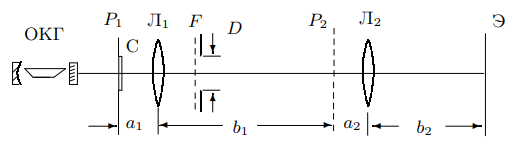
\includegraphics[width = 0.9\textwidth]{Experimental setup.png}
    \caption{Схема экспериментальной установки -- модель проекционного микроскопа}
\end{figure}

Излучение лазера (ОКГ) почти перпендикулярно падает на сетку $С$, установленную вблизи фокальной плоскости линзы $Л_1$ -- объектива микроскопа. В нашей модели линза $Л_1$ выбирается достаточно длиннофокусной ($f \approx 10 $ см), т. к. размер первичного изображения в фокальной плоскости $F$ должен быть не слишком малым, чтобы дополнительными диафрагмами можно было влиять на вторичное изображение в плоскости $P_2$. Вторичное изображение из плоскости $P_2$ проецируется на экран $Э$ линзой $Л_2$.

Изображение сетки периодически повторяется -- $репродуцируется$ -- в пространстве между сеткой и первой линзой, поэтому для того, чтобы среди множества репродуцированных изображений сетки можно было выделить её геометрическое изображение, на одну из сеток наложена тонкая проволочка, т.е. непериодический объект, изображение которого не репродуцируется.

В фокальной плоскости $F$ могут быть установлены диафрагмы -- щелевая или ирисовая (отверстие с переменным диаметром) и различного рода маски (препятствия).

Как видно из соотношения \eqref{eq: min resolving distance}, минимально разрешимый шаг решетки или сетки определяется апертурным углом $u$ объектива. Имея набор сеток с различными периодами $d$ и изменяя апертурный угол объектива с помощью щелевой диафрагмы, можно экспериментально проверить соотношение \eqref{eq: min resolving distance}.

В данной работе период сеток рассчитывается двумя способами: в первом способе (дифракция Фраунгофера) -- расстояние между дифракционными максимумами на экране измеряется при помощи линейки, а затем по формуле решетки \eqref{eq: max condition Fraunhofer diffraction} определяется ее период; во втором способе период определяется по увеличенному с помощью модели микроскопа изображению сетки на экране. 

С помощью откалиброванных таким образом сеток определяется разрешающая способность микроскопа. Для этого в задней фокальной плоскости $F$ объектива устанавливается щелевая диафрагма с микрометрическим винтом и подбирается ее минимальный размер, при котором еще видно изображение сетки на экране (щель пропускает максимумы с $m = 0$ , $ \pm 1$). По размеру диафрагмы и фокусному расстоянию объектива рассчитывается апертурный угол $u$ и проверяется соотношение \eqref{eq: min resolving distance}.

Для выполнения последней части работы ширина вспомогательной щели и угол наклона к оси системы подбираются так, чтобы на экране вместо изображения сетки получалось изображение решётки, расположенной наклонно, т. е. осуществлялась \textit{пространственная фильтрация}. Если сетку и щель поменять местами, то соответствующим подбором сетки можно «рассечь» первичное изображение так, что изображение щели на экране будет многократно повторяться -- \textit{мультиплицироваться}.

\section{Обработка данных}
Все измерения в работе проводятся с помощью лазера зелёного света с длиной волны $\lambda = 532$ нм. В работе используются три различных дифракционных сетки с различными периодами.  

\subsection{Определение периода решёток по их пространственному спектру}
\begin{enumerate}
    \item 
    Соберём схему для наблюдения на экране дифракции Фраунгофера.
    \item 
    Для каждой из трёх сеток измерим расстояния между соседними дифракционными максимумами. Результаты представлены в таблице ниже.
    \begin{table}[H]\label{tab: distance between maximums}
        \centering
        \begin{tabular}{|
            >{\columncolor[HTML]{FFFFFF}}c |
            >{\columncolor[HTML]{FFFFFF}}c |
            >{\columncolor[HTML]{FFFFFF}}c |
            >{\columncolor[HTML]{FFFFFF}}c |}
            \hline
            {\color[HTML]{000000} № решётки} &
              {\color[HTML]{000000} 1} &
              {\color[HTML]{000000} 2} &
              {\color[HTML]{000000} 3} \\ \hline
            {\color[HTML]{000000} $\Delta$, мм} &
              {\color[HTML]{000000} $76 \pm 1$} &
              \cellcolor[HTML]{FFFFFF}{\color[HTML]{000000} $30 \pm 1$} &
              \cellcolor[HTML]{FFFFFF}{\color[HTML]{000000} $15 \pm 1$} \\ \hline
        \end{tabular}
        \caption{Расстояния между максимумами дифракционной картины}
    \end{table}
    \item
    Далее запишем расстояние от сетки до экрана:
    \[L = (141,0 \pm 0,1)\text{ см}\]
    Погрешность измерения расстояний $\sigma = 1$ мм.
    \item
    Используя формулу \eqref{eq: max condition Fraunhofer diffraction} и измеренные ранее расстояния, рассчитаем периоды решёток. Для этого примем $\varphi = \Delta / L$.
    \begin{table}[H]\label{tab: grid periods 1}
        \centering
        \begin{tabular}{|
            >{\columncolor[HTML]{FFFFFF}}c |
            >{\columncolor[HTML]{FFFFFF}}c |
            >{\columncolor[HTML]{FFFFFF}}c |
            >{\columncolor[HTML]{FFFFFF}}c |}
            \hline
            {\color[HTML]{000000} № решётки}           & {\color[HTML]{000000} 1}             & {\color[HTML]{000000} 2}             & {\color[HTML]{000000} 3}              \\ \hline
            {\color[HTML]{000000} $d$, мкм}            & {\color[HTML]{000000} $9,9 \pm 0,1$} & {\color[HTML]{000000} $25,0\pm 0,6$} & {\color[HTML]{000000} $50,0 \pm 2,4$} \\ \hline
            {\color[HTML]{000000} $\varepsilon$, $\%$} & {\color[HTML]{000000} 1,0}           & {\color[HTML]{000000} 2,4}           & {\color[HTML]{000000} 4,8}            \\ \hline
        \end{tabular}
        \caption{Периоды дифракционных решёток}
    \end{table}
    Погрешности величин рассчитывались по формуле 
    \[\sigma_d = \sqrt{\bigg(\frac{\lambda}{\Delta}\bigg)^2 + \bigg(\frac{\lambda}{\Delta^2}\bigg)^2}\sigma.\]
\end{enumerate}

\subsection{Определение периода решёток по изображению, увеличенному с помощью модели микроскопа}
\begin{enumerate}
    \item 
    Соберём модель проекционного микроскопа согласно рис. 4. Запишем параметры установки.
    \begin{table}[H]\label{tab: exp setup params}
        \centering
        \begin{tabular}{|
        >{\columncolor[HTML]{FFFFFF}}c |
        >{\columncolor[HTML]{FFFFFF}}c |
        >{\columncolor[HTML]{FFFFFF}}c |
        >{\columncolor[HTML]{FFFFFF}}c |
        >{\columncolor[HTML]{FFFFFF}}c |}
        \hline
        {\color[HTML]{000000} Параметр} &
          {\color[HTML]{000000} $a_1$} &
          {\color[HTML]{000000} $a_2$} &
          {\color[HTML]{000000} $b_1$} &
          {\color[HTML]{000000} $b_2$} \\ \hline
        {\color[HTML]{000000} Значение, мм} &
          \cellcolor[HTML]{FFFFFF}{\color[HTML]{000000} $115 \pm 1$} &
          {\color[HTML]{000000} $25 \pm 1$} &
          {\color[HTML]{000000} $795 \pm 1$} &
          {\color[HTML]{000000} $490 \pm 1$} \\ \hline
        \end{tabular}
        \caption{Параметры установки}
    \end{table}
    Погрешность измерения расстояний $\sigma = 1$ мм.
    \item 
    Измерим периоды изображений сеток на экране, занесём результаты в таблицу.
    \begin{table}[H]\label{tab: grid distance}
        \centering
        \begin{tabular}{|
            >{\columncolor[HTML]{FFFFFF}}c |
            >{\columncolor[HTML]{FFFFFF}}c |
            >{\columncolor[HTML]{FFFFFF}}c |
            >{\columncolor[HTML]{FFFFFF}}c |}
            \hline
            {\color[HTML]{000000} № решётки}    & {\color[HTML]{000000} 1}             & {\color[HTML]{000000} 2}             & {\color[HTML]{000000} 3}           \\ \hline
            {\color[HTML]{000000} $\Delta$, мм} & {\color[HTML]{000000} $1,3 \pm 0,1$} & {\color[HTML]{000000} $3,6 \pm 0,1$} & {\color[HTML]{000000} $7 \pm 0,1$} \\ \hline
        \end{tabular}
        \caption{Периоды изображений сеток на экране}
    \end{table}
    \item
    Для всей системы увеличение составляет $b_1 b_2 / a_1 a_2$. Таким образом, используя измерения из прошлого пункта, рассчитаем периоды решёток вторым способом: $d = a_1 a_2 / b_1 b_2 \cdot \Delta$.
    \begin{table}[H]\label{tab: grid periods 2}
        \centering
        \begin{tabular}{|
            >{\columncolor[HTML]{FFFFFF}}c |
            >{\columncolor[HTML]{FFFFFF}}c |
            >{\columncolor[HTML]{FFFFFF}}c |
            >{\columncolor[HTML]{FFFFFF}}c |}
            \hline
            {\color[HTML]{000000} № решётки}           & {\color[HTML]{000000} 1}             & {\color[HTML]{000000} 2}             & {\color[HTML]{000000} 3}              \\ \hline
            {\color[HTML]{000000} $d$, мкм}            & {\color[HTML]{000000} $9,6 \pm 0,8$} & {\color[HTML]{000000} $26,6\pm 1,3$} & {\color[HTML]{000000} $51,7 \pm 2,2$} \\ \hline
            {\color[HTML]{000000} $\varepsilon$, $\%$} & {\color[HTML]{000000} 8,3}           & {\color[HTML]{000000} 4,9}           & {\color[HTML]{000000} 4,3}            \\ \hline
        \end{tabular}
        \caption{Периоды дифракционных решёток}
    \end{table}
    Погрешности величин рассчитывались по формуле 
    \[\sigma_d^2 = \bigg(\frac{a_2\Delta}{b_1 b_2}\bigg)^2 \sigma_{a_1}^2 + \bigg(\frac{a_1\Delta}{b_1 b_2}\bigg)^2 \sigma_{a_2}^2 +
    \bigg(\frac{a_2 a_1\Delta}{b_1^2 b_2}\bigg)^2 \sigma_{b_1}^2 +
    \bigg(\frac{a_2 a_1\Delta}{b_1 b_2^2}\bigg)^2 \sigma_{b_2}^2 + 
    \bigg(\frac{a_2 a_1}{b_1 b_2^2}\bigg)^2 \sigma_\Delta^2.\]
    
\end{enumerate}

\subsection{Определение периода решёток по оценке разрешающей способности микроскопа}
\begin{enumerate}
    \item
    Добавим к установке щелевую диафрагму с микрометрическим винтом, поместим её в фокальную плоскость $F$ линзы $Л_1$. 
    \item
    Для каждой решётки определим минимальный размер диафрагмы $D$, при котором на экране ещё видно изображение сетки (при меньших размерах щели изображение будет выглядеть как одномерная решётка). Результаты измерений приведены в таблице ниже.
    \begin{table}[H]\label{tab: gap width}
        \centering
        \begin{tabular}{|
            >{\columncolor[HTML]{FFFFFF}}c |
            >{\columncolor[HTML]{FFFFFF}}c |
            >{\columncolor[HTML]{FFFFFF}}c |
            >{\columncolor[HTML]{FFFFFF}}c |}
            \hline
            {\color[HTML]{000000} № решётки} & {\color[HTML]{000000} 1}           & {\color[HTML]{000000} 2}           & {\color[HTML]{000000} 3}           \\ \hline
            {\color[HTML]{000000} $D$, мкм}  & {\color[HTML]{000000} $2660 \pm 50$} & {\color[HTML]{000000} $1000 \pm 50$} & {\color[HTML]{000000} $500 \pm 50$} \\ \hline
        \end{tabular}
        \caption{Критическая ширина щели для разных решёток}
    \end{table}
    \item
    Используя формулу \eqref{eq: min resolving distance}, рассчитаем период для каждой из решёток третьим способом. Для этого запишем значение фокусного расстояния линзы $Л_1$:
    \[f = 25 \text{ мм.}\]
    \begin{table}[H]\label{tab: d results 3}
        \centering
        \begin{tabular}{|
            >{\columncolor[HTML]{FFFFFF}}c |
            >{\columncolor[HTML]{FFFFFF}}c |
            >{\columncolor[HTML]{FFFFFF}}c |
            >{\columncolor[HTML]{FFFFFF}}c |}
            \hline
            {\color[HTML]{000000} № решётки} & {\color[HTML]{000000} 1}              & {\color[HTML]{000000} 2}              & {\color[HTML]{000000} 3}              \\ \hline
            {\color[HTML]{000000} $d$, мкм}  & {\color[HTML]{000000} $10,0 \pm 0,2$} & {\color[HTML]{000000} $26,6 \pm 1,3$} & {\color[HTML]{000000} $53,2 \pm 5,3$} \\ \hline
        \end{tabular}
        \caption{Периоды дифракционных решёток}
    \end{table}
\end{enumerate}

%\subsection{Пространственная фильтрация и мультиплицирование}
%\begin{enumerate}
%    \item 
%\end{enumerate}

%\newpage
\section{Вывод}
В данной работе было проведено исследование разрешающей способности микроскопа методом Аббе, а также определены периоды дифракционных решёток трёмя различными способами:
\begin{itemize}
    \item
    по их пространственному спектру
    
    \item
    по изображению, увеличенному с помощью модели микроскопа
    
    \item
    по оценке разрешающей способности микроскопа
    
\end{itemize}

%%%%%%%%%%%%%%%%%%%%%%%%% Графики
\newpage
\begin{figure}[H]\label{fig: d(D-1)}
    \centering
    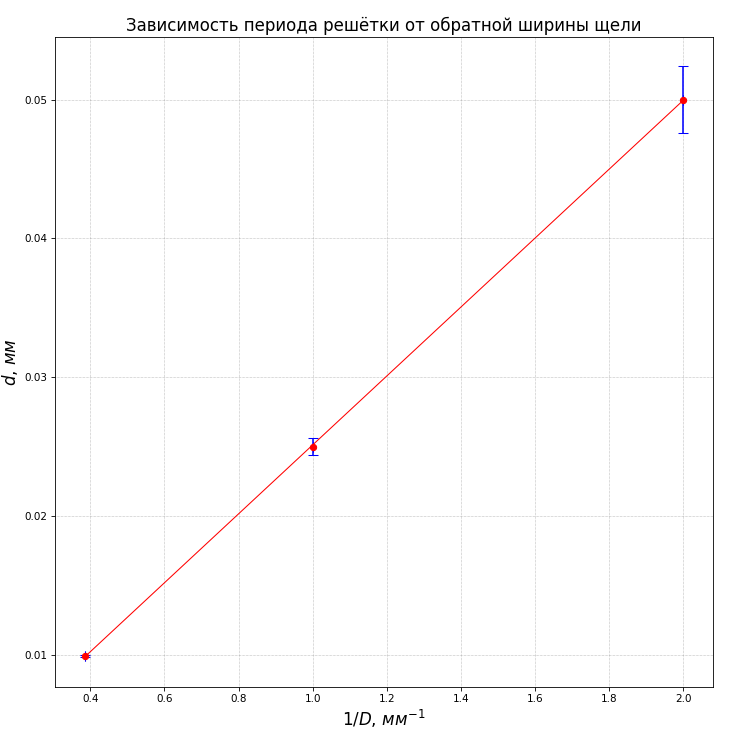
\includegraphics[width = 0.9\textwidth]{d(D-1).png}
\end{figure}

%%%%%%%%%%%%%%%%%%%%%%%%%
\end{document}
